%kelompok 3 kelas 3B
%Diana Satima Gistivani 1154018
%M.AMRAN HAKIM SIREGAR 1154106
%INDAH RAHMAWATI 1154070



\section{data vektor}
  Data vektor dalam Sistem Informasi Geografis. dalam  data vektor bumi direpresentasikan sebegai suatu  mosaic yang terdiri dari garis (arclline), polygon (dareah yang dibatasi oleh garis yang berawal dan berakhir pada titik yang sama), titik/point (node yang memiliki label),  dan nodes (titik perpotongan antara dua buah garis).
  
 \section{data raster}
 Data raster merupakan data yang disimpan dalam bentuk kotak segi empat (grid)
atau sel sehingga terbentuk suatu ruang yang teratur.Pada data raster,objek geografis dipresentasikan sebagai struktur sel grid yang disebut sebagai pixel (picture element).Definisi gambar tergantung pada ukuran pixel-nya,semakin kecil ukuran permukaan bumi yang dipresentasikan oleh sel,semakin tinggi ukuran permukaannya.

\begin{figure}[ht]
\centerline{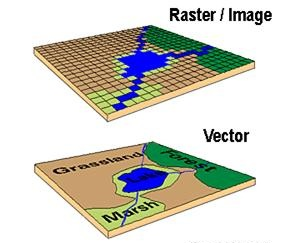
\includegraphics[width=1\textwidth] {figures/vektor01.JPG}}
\caption{tampilan dari data vektor dan data raster}
\label{vektor01}
\end{figure}
Pada gambar \ref{vektor01} ditampilkan gambar data vector dan juga data raster yang memiliki perbedaan dalam segi tampilan.

\subsection
  Model data vektor sendiri merupakan model yang banyak digunakan, model ini berbasis pada titik (points) dengan nilai koordinat (x,y) untuk membangun objek spasialnya. 
\subsection {Perbedaan Data Vektor dan Raster}
Sistem Informasi Geografis : Prinsip Dasar dan Pengembangan Aplikasi
\subsection {Objek pada datavektor}
\begin{figure}[ht]
\centerline{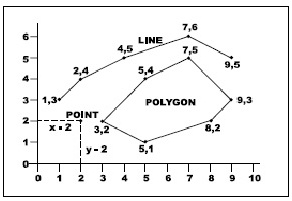
\includegraphics[width=1\textwidth] {figures/vektor02.JPG}}
\caption{tampilan dari data vektor dan data raster}
\label{vektor02}
\end{figure}
Sesuai pada gambar \ref{vektor02} 
\begin{enumerate}
Objek yang dibangun terbagi menjadi tiga bagian lagi, yaitu berupa titik (point), garis (line), dan area (polygon). 
\item titik (point) merupakan representasi grafis yang paling sederhana pada suatu objek. Titik tidak mempunyai dimensi tetapi dapat ditampilkan dalam bentuk symbol baik pada peta maupun dalam layar monitor.
\item garis (line) merupakan bentuk linear yang menghubungkan dua ataui lebih titik dan merepresentasikan objek dalam satu dimensi. 
\item Area (polygon) merupakan representasi objek dalam dua dimensi.
\end{enumerate}

\subsection{kelebihan dan kekurangan data vektor}
\begin{enumerate}
\item
Kelebihan data vektor di bandingkan data raster
data vektor relatif lebih ekonomis dalam hal ukuran file dan presisi dalam lokasi, tetapi sangat sulit untuk digunakan dalam komputasi matematik. 

\item
kekurangan data vector dibandingkan data raster
terdapat keterbatasan masalah akurasi dan presisi data terutama dalam menentukan ukuran piksel. Data vector memiliki keterbatasan dalam ukuran penyimpanan atau kapasitas hasil.
\end{enumerate}


